\iffalse
\title{}
\author{EE24BTECH11053 - S A Aravind Eswar
}
\chapter{2019}
\section{ee}
\fi
    \item The probablity of a resistor being defective is 0.02. There are 50 such resistors in a circuit. The probability of two or more defective resistors in the circuit (round off to two decimal places) is \underline{\hspace{3cm}}.\hfill{[2019 - EE]}
    \item A 0.1 $\mu$F capacitor charged to 100 $V$ is discharged through  1 $k\Omega$ resistor. The time in $ms$ (round off to two decimal places) required for the voltage across the capacitor to drop to 1 $V$ is \underline{\hspace{3cm}}.\hfill{[2019 - EE]}
    \item The current $I$ flowing in the circuit shown below in amperes is \underline{\hspace{3cm}}.\hfill\\\strut\hfill{[2019 - EE]}\\
        \begin{center}
            \begin{circuitikz}
\draw (0,3) to[R,l_=50$\Omega$] (0,1.5) to[battery1, l=200 V] (0,0) -- (8,0) (8,3) to[R, i=$I$] (8,0) (8,3)-- (0,3) (2,3) to[R, l_=40$\Omega$] (2,1.5) to[battery1, l=160 V] (2,0) (4,0) to[battery1, l_ = 100 V] (4,1.5) to[R, l = 25 $\Omega$] (4,3) (6,0) to[battery1, l_=80 V] (6,1.5) to[R=, l=20 $\Omega$] (6,3) ;
\end{circuitikz}


        \end{center}
    \item The volatage across and the current through a load are expressed as follows 
        \begin{align*}v(t) &= -170 \sin \brak{377t - \frac{\pi}{6}} V\\i(t) &= 8\cos\brak{377t+\frac{\pi}{6}} A\end{align*}
        The average power in watts (round off to one decimal place) consumed by the load is \underline{\hspace{3cm}}.\hfill{[2019 - EE]}
    \item The magnetic circuit shown below has uniform cross-section area and air gap of 0.2$cm$. The mean path length of the core is 40$cm$. Assume that leakage and fringing fluxes are negligible. When the core relative permeability is assumed to be infinite, the magnetic flux density computed in the air gap is 1 tesla. With the same Ampere-turns, if the core relative permeability is assumed to be 1000 (linear), the flux density in tesla (round off the three decimal places) calulated in the air gap is \underline{\hspace{3cm}}. \hfill{[2019- EE]}
        \begin{center}
            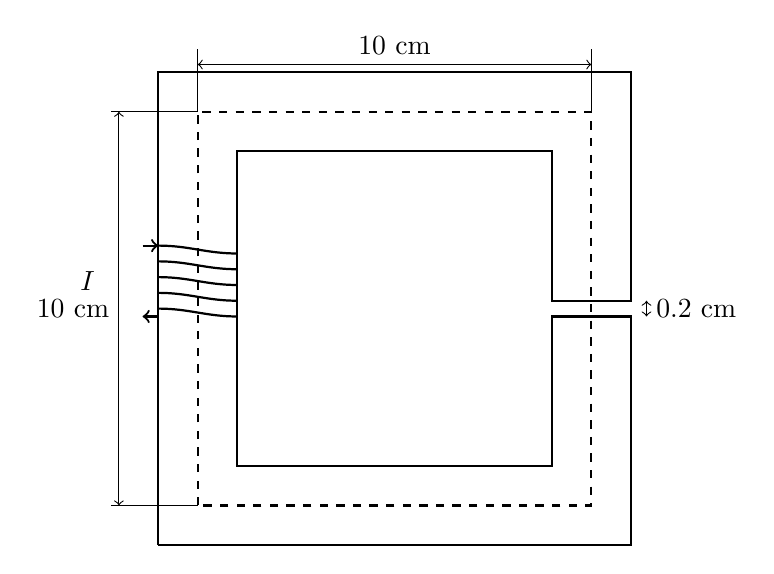
\begin{tikzpicture}
    % Define dimensions
    \def\outerwidth{5}    % Outer square width (cm)
    \def\innerwidth{9.6}   % Inner square width (10 - 0.4, considering 0.2 cm gap on each side)
    \def\gap{0.2}          % Gap size (cm)
    \def\coilspacing{0.2}  % Coil spacing (cm)
    \def\coilloops{5}      % Number of coil loops

    % Outer square
    \draw[thick] (0,0) -- (6,0) -- (6,2.9) -- (5,2.9) -- (5,1) -- (1,1) -- (1, 5) -- (5, 5) -- (5,3.1) -- (6,3.1) -- (6, 6) -- (0, 6) -- (0,0);
    %\draw[thick] 
    \draw (0.5, 5.5) -- (0.5, 6.3);
    \draw (5.5, 5.5) -- (5.5, 6.3);
    \draw (.5, .5) -- (-.6, 0.5);
    \draw (.5, 5.5) -- (-.6, 5.5);
    % Inner square
    \draw[thick, dashed] (0.5, 0.5) rectangle (5.5,5.5);

    % Winding with current I
    \foreach \i in {1,...,\coilloops} {
        \draw[thick] (1, 4 - \i * \coilspacing - \coilspacing/2) to[out=180, in=0] 
            (0, 4 - \i * \coilspacing) ;
    }

    % Label the current I
    \node at (-.9, 3.35) {$I$};

    % Dimensions
    \draw[thick][->] (-0.2, 3.8) -- (0, 3.8);
    \draw[thick][<-] (-0.2, 2.9) -- (0, 2.9);
    \draw[<->] (0.5, 6.1) -- (5.5, 6.1) node[midway, above] {10 cm};
    \draw[<->] (-.5, 0.5) -- (-.5, 5.5) node[midway, left] {10 cm};
    \draw[<->] (6.2, 2.9) -- (6.2, 3.1) node[midway, right] {0.2 cm};
\end{tikzpicture}


        \end{center}
\item A single-phase transformer of rating 25$kVA$, supplies a 12$kW$ load at power factor 06 lagging. The additional load at unirt power factor in $kW$(round off to two decimal places) that may be added before this transformer exceeds it's rated $kVA$ is \underline{\hspace{3cm}}. \hfill{[2019 - EE]}
\item A 220$V$ CD shunt motor takes 3$A$ at no-load. It draws 25$A$ when running at full-load at 1500 rpm. The armature and shunt resistances are 0.5 $\Omega$ and 220 $\Omega$, respectively. The no-load speed in rpm (round off to two decimal places) is \underline{\hspace{3cm}}. \hfill{[2019 - EE]}
\item A delta-connected, 3.7 $kW$, 400 $V$(line), three-phase, 4-pole, 50-$Hz$ squirrel-cage induction motor has the following equivalent circuit parameters per phase referred to the stator: $R_1 - 5.39 \Omega, R_2 = 5.72 \Omega, X_1 = X_2 = 8.22 \Omega$. Neglet shunt branch in the equivalent circuit. The starting line current in amperes (round off the two decimal places) when it is connected to a 100 $V$ (line), 10 $Hz$, three-phase AC source is \underline{\hspace{3cm}}. \hfill{[2019 - EE]}

\item A 220 $V$ (line), three-phase, Y-connected, synchronous motor has a synchorous impedance of $(0.25 + j2.5)\Omega$/phase. The motor draws the rated current of 10 $A$ at 0.8 $pf$ leading. The rms value of line-to-line internal voltage in volts (round off to two decimal places) is \underline{\hspace{3cm}}. \hfill{[2019 - EE]}
\item A three-phase 50 $Hz$, 400 $kV$ transmission line is 300 $km$ long. The line inductance is 1 $mH/km$ per phase, and the capacitance is 0.01 $\mu F/km$ per phase. The line is under open circuit condition at the receiving end and energized with 400 $kV$ at the sending end, the receiving end line voltage in $kV$ (round off to two decimal places) will be \underline{\hspace{3cm}}. \hfill{[2019 - EE]}
\item A 30 $kV$, 50 $Hz$, 50 $MVA$ generator has the positive, negative, and zero sequence reactances of 0.25 $pu$, 0.15 $pu$, and 0.05 $pu$, respectively. The neutral of the generator is grounded with a reactance so that the fault current for a bolted LG fault and that of a bolted three-phase fault at the generator terminal are equal. The value of grounding reactance in ohms (round off to one decimal place) is \underline{\hspace{3cm}}. \hfill{[2019 - EE]}
\item In the single machine infinite bus system shown below, the generator is delivering the real power of 0.8 $pu$ at 0.8 power factor lagging to the infinite bus. The power angle of the generator in degrees (round off to one decimal place) is \underline{\hspace{3cm}}. \hfill{[2019 - EE]}
    \begin{center}
        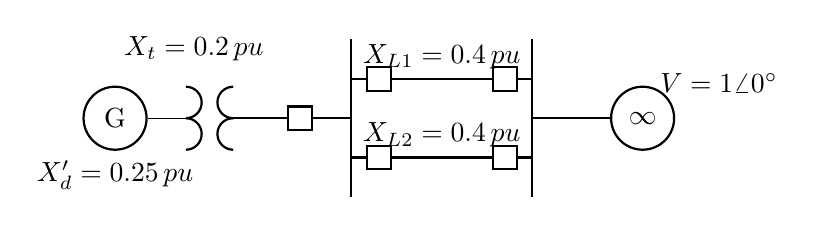
\begin{tikzpicture}
    % Generator
    \node[circle, draw, thick, minimum size=0.8cm, inner sep=0] (G) at (0,0) {G};
    \node[below] at (G.south) {$X_d' = 0.25 \, \text{pu}$};

    % Transformer reactance Xt
    \draw (G.east) -- ++(0.5, 0);
    \draw[thick] (1.5,0.4) arc[start angle=90,end angle=270,radius=0.2cm];
    \draw[thick] (1.5,-0) arc[start angle=90,end angle=270,radius=0.2cm];
    \draw[thick] (0.9,0) arc[start angle=270,end angle=450,radius=0.2cm];
    \draw[thick] (0.9,-.4) arc[start angle=270,end angle=450,radius=0.2cm];
    \node[above] at (1,0.6) {$X_t = 0.2 \, \text{pu}$};

    % Transmission line
    \draw[thick] (1.5,0) -- (2.2,0);
    \draw[thick] (2.2, -0.15) rectangle (2.5, 0.15);
    \draw[thick] (2.5, 0) -- (3, 0);
    \draw[thick] (3,-1) -- (3,1);  % Bus line

    % Inductors X_L1 and X_L2
    % Upper inductor X_L1
    \draw[thick] (3,0.5) -- (3.2, 0.5);
    \draw[thick] (3.2, 0.35) rectangle (3.5, 0.65);
    \draw[thick] (3.5,0.5) -- (4.8,0.5) node[midway, above] {$X_{L1} = 0.4 \, \text{pu}$};
    \draw[thick] (4.8,0.35) rectangle (5.1,0.65);
    \draw[thick] (5.1,0.5) -- (5.3,0.5);
    
    % Lower inductor X_L2
    \draw[thick] (3,-0.5) -- (3.2, -0.5);
    \draw[thick] (3.2, -0.35) rectangle (3.5, -0.65);
    \draw[thick] (3.5,-0.5) -- (4.8,-0.5) node[midway, above] {$X_{L2} = 0.4 \, \text{pu}$};
    \draw[thick] (4.8,-0.35) rectangle (5.1,-0.65);
    \draw[thick] (5.1,-0.5) -- (5.3,-0.5);

    % Right side bus line
    \draw[thick] (5.3,-1) -- (5.3,1);
    
    % Infinite bus
    \draw[thick] (5.3,0) -- ++(1,0);
    \node[circle, draw, thick, minimum size=0.8cm, inner sep=0] (inf) at (6.7,0) {};
    \node at (inf) {\(\infty\)};
    \node[above right] at (6.8,0.2) {$V = 1 \angle 0^\circ$};
\end{tikzpicture}

    \end{center}
    \item In a 132 $kV$ system, the series inductance up to the point of circuirbreaker locationis 50 mH. The shunt capasitance at the circuit breaker terminal is 0.05 $\mu F$. The critical value of resistance in ohm required to be connected across the circuit breaker contacts which will give no transient oscillation is. \underline{\hspace{3cm}}.\hfill{[2019 - EE]}


